\chapter{Background: Quality-control mechanisms on Wikipedia}
\label{chap:background}

\begin{comment}
- algorithmic governance
- code is law
\end{comment}

In the present chapter we study scientific literature on quality control mechanisms in Wikipedia in order to better understand the role of edit filters in this ecosystem.
There are works on vandalism detection in general/detection of unencyclopedic content~\cite{PotSteGer2008}, %TODO is this significant? are there really that many "in general"?
as well as several articles dedicated to bots and the role they play in mainataining quality on Wikipedia~\cite{GeiHal2013}, \cite{Geiger2014}, \cite{GeiHal2017}, \cite{GeiRib2010}, \cite{HalRied2012}, \cite{Livingstone2016}, \cite{MueDoHer2013}, \cite{MuellerBirn2014}...,
a couple which discuss combating vandalism by means of semi-automated tools such as Huggle, Twinkle and STiki~\cite{GeiRib2010}, \cite{HalRied2012}, \cite{WestKanLee2010}, \cite{GeiHal2013} ...
and also some accounts on the emerging machine learning service ORES~\cite{HalTar2015}, \cite{HalGeiMorSarWig2018}.
Time and again, the literature refers also to more ``manual'' forms of quality control by editors using watchlists to keep an eye on articles they care about or even accidentially discovering edits made in bad faith~\cite{Livingstone2016}, \cite{AstHal2018}.
There is one mechanism though that is very ostentatiously missing from all these reports: edit filters.

\begin{figure}
\centering
  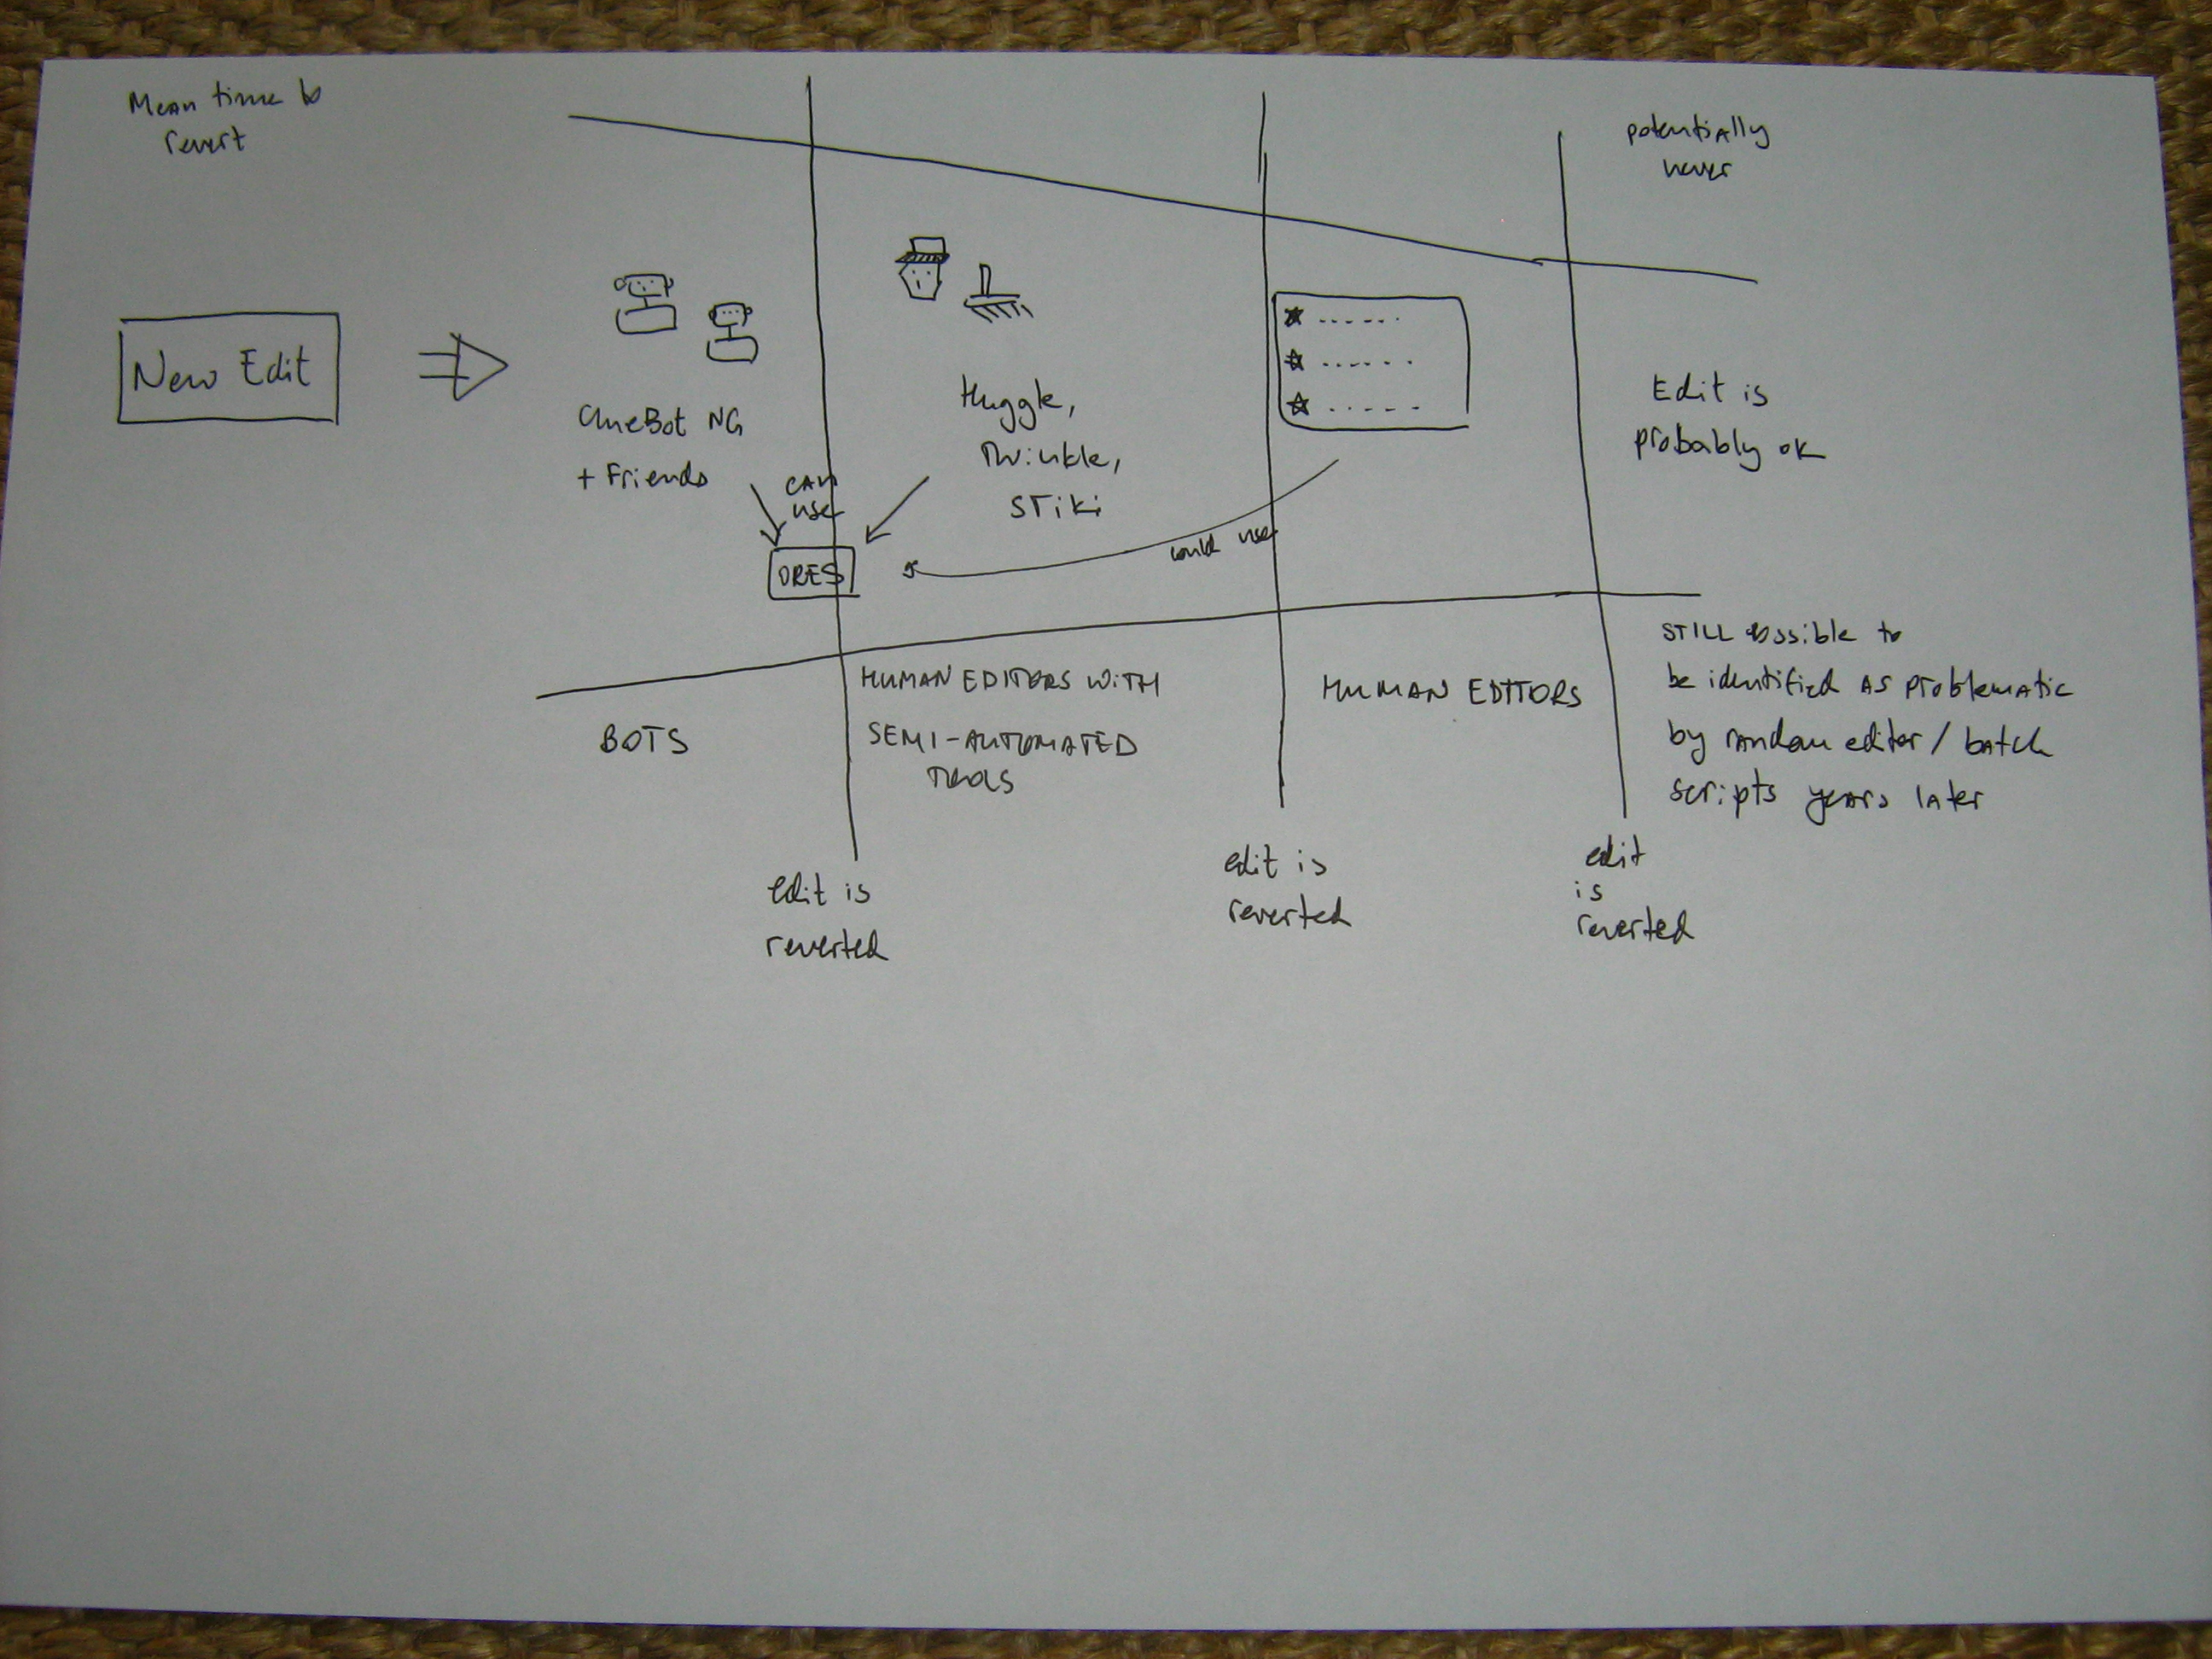
\includegraphics[width=0.9\columnwidth]{pics/funnel-diagramm-no-filters.JPG}
  \caption{State of the scientific literature: edit filters are missing from the quality control frame}~\label{fig:funnel-no-filters}
\end{figure}
%TODO merge with rise and decline graphic from~\cite{HalGeiMorRied2013}

At first, scientific studies on Wikipedia largely ignored algorithmic quality control mechanisms.
Their contribution to the encyclopedia and therefore their impact were considered insignificant. %quote?
This has gradually changed since around 2009 when the first papers specifically dedicated to bots (and later semi-automated tools) were published.
In 2010, Geiger and Ribes insistently highlighted that the scientific community could no longer ingore(syn) these mechanisms as insignificant(syn) or noise in the data~\cite{GeiRib2010}.
For one, their (the mechanisms') relative usage has continued to increase since they were first introduced, and in an observed two-months period in 2009 bots made 16.33\% of all edits~\cite{Geiger2009}.

Others were worried it was getting increasingly intransparent how the encyclopedia functions and not only ``[k]eeping traces obscure help[ed] the powerful to remain in power''~\cite{ForGei2012} but entry barriers for new users were gradually set higher, since they not only had to learn to use/interact with a myriad of technical tools/.. (learn wikisyntax, ..) but also navigate their ground in a complex system with a decentralised socio-technical mode of governance~\cite{Geiger2017}.
Ford and Geiger even cite a case where an editor was not sure whether a person deleted their articles or a bot~\cite{ForGei2012}.

What is more, Geiger and Ribes argue, the algorithmic quality control mechanisms change the system not only in matter of scale (using bots/tools is faster, hence more reverts are possible) but in matter of substance: how everything interacts with each other~\cite{GeiRib2010}.
On the grounds of quality control specifically, the introduction of tools (and bots) was fairly revolutionary:
they enabled efficient patrolling of articles by users with little to no knowledge about the particular topic.
Thanks to Wikipedia's particular software architecture, this is possible even in the most ``manual'' quality control work (e.g. using watchlists to patrol articles): representing information changes via diffs allows editors to quickly spot content that deviates from its immediate context~\cite{GeiRib2010}.

\begin{comment}
%Why is it important we study these mechanisms?
- their relative usage increases/has increased since they were first introduced
    \cite{GeiRib2010}
    "at present, bots make 16.33\% of all edits."
    %TODO more recent data? the last month argument via recentchanges (vgl \cite{Geiger2017}) doesn't hold here; couldn't find anything useful unfortunately :(
- the whole ecosystem is not transparent, especially for new users (see~\cite{ForGei2012}: "As it is, Kipsizoo is not even
sure whether a real person who deleted the articles or a bot."
"Keeping traces obscure help the powerful to remain in power"~\cite{ForGei2012}
- higher entry barriers: new users have to orientate themselves in the picture and learn to use the software (decentralised mode of governance, often "impenetrable for new editors", vgl~\cite{ForGei2012})

!! tools not only speed up the process but:
    "These tools greatly lower certain barriers to participation and render editing
    activity into work that can be performed by "average
    volunteers" who may have little to no knowledge of the
    content of the article at hand"

%Numbers
\cite{GeiRib2010}
Check Figure 1: Edits to AIV by tool (in the meantime 10 years old. is there newer data on the topic??)
not really, see:
\cite{Geiger2017}
"In the English-lan-
guage Wikipedia, 22 of the 25 most active editors (by
number of edits) are bot accounts, and July 2017, they
made about 20\% of all edits to encyclopedia articles."
Geiger's evidence:
https://quarry.wmflabs.org/query/20703
Percent of bot edits in previous month (enwiki, all pages)
\begin{verbatim}
is_bot	edits	Percentage of all edits
0	    7619466	79.4974
1	    1965083	20.5026
\end{verbatim}

https://quarry.wmflabs.org/query/20704
Percent of bot edits in previous month (enwiki, articles only)
\begin{verbatim}
is_bot	edits	Percentage of all edits
0	    4273810	80.2025
1	    1054966	19.7975
\end{verbatim}

However, a month is a relatively small period and you can't make an argument about general trends based on it.
For instance, these same quarries ran on April 12, 2019 render following results:
https://quarry.wmflabs.org/query/35104
Percent of bot edits in previous month (enwiki, all pages)
\begin{verbatim}
is_bot	edits	Percentage of all edits
0	    6710916	89.7318
1	    767948	10.2682
\end{verbatim}

https://quarry.wmflabs.org/query/35105
Percent of bot edits in previous month (enwiki, articles only)
\begin{verbatim}
is_bot	edits	Percentage of all edits
0	    3426624	92.1408
1	    292274	7.8592
\end{verbatim}
\end{comment}


\section{Bots}

%todo also mention bot papers that discuss more general aspects of bots?
According to literature, bots constitute the first line of defence against malicious edits~\cite{GeiHal2013}. %TODO but that's actually not true! edit filters are triggered first. Comment on this!
They are also undoubtedly the vandal fighting mechanism studied most in depth by the scientific community. %TODO replace "vandal fighting" with "quality control"?

Geiger and Ribes~\cite{GeiRib2010} define bots as
``fully-automated software
agents that perform algorithmically-defined tasks involved
with editing, maintenance, and administration in Wikipedia.''

%todo summarise aspects of bot papers:
trace enthnography and banning of vandals~\cite{GeiRib2010}
indepth analysis of ClueBot NG, and its place within vandal fighting infrastructure~\cite{GeiHal2013}
historical review of bots' and semi-automated tools' involvement in vandal fighting\cite{HalRied2012}
... (smth else??)

Further bots involved in vandal fighting discussed by the literature include (besides ClueBot NG~\cite{GeiHal2013}, \cite{HalRied2012},)
XLinkBot~\cite{HalRied2012},
HBC AIV Helperbots~\cite{HalRied2012}, \cite{GeiRib2010},
MartinBot, AntiVandalBot~\cite{HalRied2012},
AWB, DumbBOT, EmausBot~\cite{GeiHal2013}.

Very crucial for the current analysis will also be Livingstone's observation in the preamble to his interview with the first large scale bot operator Ram-man that
``In the Wikimedia software, there are tasks that do all sorts of things [...].
If these things are not in the software, an external bot could do them. [...]
The main difference is where it runs and who runs it''~\cite{Livingstone2016}.

This thought/note is also scrutinised by Geiger~\cite{Geiger2014} who examines in detail what the difference and repercussions are of code that is part of the core software and code that runs alongside it (such as bots). %TODO more detail: so what are they?

- "inofficial", run and maintained by the community
    \cite{GeiRib2010}
    "often-unofficial technologies have fundamentally
    transformed the nature of editing and administration in
    Wikipedia"
    "Of note is the fact that these tools are largely
    unofficial and maintained by members of the Wikipedia
    community."

\begin{comment}
%ClueBot NG
"ClueBot\_NG uses state-of-the-art machine learning techniques to review all contributions to

ClueBot NG:
\cite{GeiHal2013}
"to scan every edit made to Wikipedia in real time"
"Built on Bayesian neural networks and trained with data
about what kind of edits Wikipedians regularly revert as
vandalism"
articles and to revert vandalism,"~\cite{HalRied2012}

%XLinkBot
"XLinkBot reverts contributions that create links to
blacklisted domains as a way of quickly and permanently dealing with spammers."~\cite{HalRied2012}

%HBC AIV Helperbots and MartinBot
"AIV Helperbot turns a simple page into a dynamic
priority-based discussion queue to support administrators in their work of identifying and
blocking vandals"~\cite{HalRied2012}


%AntiVandalBot
~\cite{HalRied2012}
"The first tools to redefine the
way Wikipedia dealt with van-
dalism were AntiVandalBot and
VandalProof."

"AntiVandalBot used a simple set
of rules and heuristics to monitor
changes made to articles, identify the
most obvious cases of vandalism, and
automatically revert them"

1st vandalism fighting bot:
"this bot made it possible, for the first
time, for the Wikipedia community
to protect the encyclopedia from
damage without wasting the time
and energy of good-faith editors"
"it
wasn’t very intelligent and could only
correct the most egregious instances
of vandalism."


Bots not patrolling constantly but instead doing batch cleanup works~\cite{GeiHal2013}:
AWB, DumbBOT, EmausBot
(also from figures: VolkovBot, WikitanvirBot, Xqbot)

\cite{GeiRib2010}
"“HBC AIV helperbot7” – automatically
removed the third vandal fighter's now-obsolete report."

\end{comment}

%TODO: gibts es vergleichbare concerns zu den Gamification concerns bei semi-automated tools bei anderen mechanismen?

\section{Semi-automated tools}

Semi-automated tools are similar to bots in the sense that they provide automated detection of potential low-quality edits.
The difference however is that with semi-automated tools humans do the final assessment and decide what happens with the edits in question.

Semi-automated tools used for vandalism fighting on Wikipedia are discussed by:
more popular/widely used:
STiki~\cite{WestKanLee2010}
\url{http://en.wikipedia.org/wiki/Wikipedia:STiki}
Huggle~\cite{GeiHal2013},~\cite{HalRied2012},\cite{GeiRib2010}
\url{https://en.wikipedia.org/wiki/Wikipedia:Huggle}
Twinkle
\url{https://en.wikipedia.org/wiki/Wikipedia:Twinkle}
AWB
\url{https://en.wikipedia.org/wiki/Wikipedia:AutoWikiBrowser}
less popular/older, mentioned in older accounts or not discussed at all (there are also more tools, see for example \url{https://en.wikipedia.org/wiki/Category:Wikipedia_counter-vandalism_tools})
VandalProof~\cite{HalRied2012}
ARV
AIV
Lupin's Anti-vandal tool~\cite{GeiRib2010}
\url{https://en.wikipedia.org/wiki/User:Lupin/Anti-vandal_tool}
"Please be aware that the original author of AVT (Lupin) is no longer active on Wikipedia. The script is very old and might stop working at any time."
"By using the RC feed to check a wiki-page's differences against a list of common vandal terms, this tool will detect many of the commonly known acts of online vandalism. "

In general, previous research seems to make a distinction of degree? between ``more'' automated tools such as Huggle and STiki and ``less'' automated ones such as Twikle~\cite{GeiHal2013}.

%Huggle
Huggle was initially released in 2008~\footnote{\url{https://en.wikipedia.org/wiki/Wikipedia:Huggle}}.
In order to use Huggle, editors need the ``rollback'' permission~\cite{HalRied2012}.
Huggle presents a pre-curated queue of edits to the user which can be classified as vandalism by a single mouse click which simultaneously takes action accordingly: the edit is reverted, the offending editor is warned~\cite{HalRied2012}.
Moreover, Huggle is able to parse the talk page of the offending user where warnings are placed in order to issue a next warning of suitable degree and also makes automated reports to AIV (Administrators Intervention Against Vandalism, explain!) if the user has exhausted the warning limit.
The software uses a set of heuristics for compiling the queue with potentially offending edits.
The defaults include placing higher edits containing large removal of content or complete blankings of a page, edits made by anonymous users or users whose edits have been reverted in the past.
Edits by users with warnings on their user talk page are sent to the top of the queue, while edits made by bots and other Huggle users are ignored altogether\cite{GeiRib2010}.
One can reconfigure the queue, however, some technical savvy and motivation is need for this and thus, as~\cite{GeiRib2010} warn, it makes certain paths of action easier to take than others.

%STiki
STiki was introduced by Andrew G. West in June 2010~\footnote{\url{https://en.wikipedia.org/wiki/Wikipedia:STiki}}.
Its defining characteristic is relying on ``spatio-temporal properties of revision metadata''~\cite{WestKanLee2010} for deciding the likelihood of an edit to be vandalism.
According to the authors, this makes the tool's vandalism detection more robust and language independent.
One of the following conditions must be fulfilled for an editor to obtain a permission to use STiki:
(1) they must have the rollback permission, or
(2) they must have made at least 1000 article edits, or
(3) they must have obtained a special permission via their talk page~\footnote{\url{https://en.wikipedia.org/wiki/Wikipedia:STiki}}.

According to~\cite{GeiHal2013} Huggle and STiki complement each other in their tasks, with Huggle users making swifter reverts and STiki users taking care of older edits.

\begin{comment}
\url{https://en.wikipedia.org/wiki/Wikipedia:STiki/leaderboard}

"Above all else, it should be emphasized that STiki is not a competition."
//compare also~\cite{HalRied2012} who warn against Wikipedia becoming gamified with vandals being "monsters"

" STiki users who operate the tool recklessly in the hope of inflating their statistics are not helping themselves or the project "

\url{https://en.wikipedia.org/wiki/Wikipedia:STiki}

"STiki is a tool available to trusted users that is used to detect and revert vandalism, spam, and other types of unconstructive edits made at Wikipedia. "

"STiki chooses edits to show to end users; if a displayed edit is judged to be vandalism, spam, etc., STiki streamlines the reversion and warning process. STiki facilitates collaboration in reverting vandalism; a centrally stored lists of edits to be inspected are served to STiki users to reduce redundant effort."

"STiki may only be used by editors with a Wikipedia account. Additionally, the account must meet some qualifications to reduce the probability of users misidentifying vandalism."

"The account must have any one of: (1) the rollback permission/right, (2) at least 1000 article edits (in the article namespace, not to talk/user pages), or (3) special permission via the talk page. We emphasize that users must take responsibility for their actions with STiki. "

"After login, users primarily interact with the GUI tool by classifying edits into one of four categories:
vandalism
good faith revert
pass
innocent "
//interestingly, at the initial tool presentation~\cite{WestKanLee2010}, there was no "good faith" option. It seemed to have been added quite promptly after though, since the screenshot of the tool on the page has the button already and claims to have been made on 28 February 2010

"Uncertainty over malice: It can be tricky to differentiate between vandalism and good-faith edits that are nonetheless unconstructive. "
\end{comment}

%Twinkle
Twinkle, a javascript based ``user interface extension that runs inside of a standard web browser''~\cite{GeiRib2010} seems to be less automated than the previous tools~\cite{GeiHal2013}.
It adds contextual links to other parts of Wikipedia which facilitates fulfilling particular tasks (rollback multiple edits, report problematic users to AIV, nominate an article for deletion) with a single click~\cite{GeiRib2010}.
A prerequisite for using Twinkle is being an autoconfirmed registered user~\footnote{\url{https://en.wikipedia.org/wiki/Wikipedia:Twinkle}}.

%TODO decide whether to elaborate more via https://en.wikipedia.org/wiki/Wikipedia:Twinkle/doc

%Lupin's anti-vandal tool
%VandalProof
Older tools which are not much used anymore include Lupin's anti-vandal tool which
``provides a real-time in-browser feed of edits made matching certain algorithms''~\cite{GeiRib2010}
and VandalProof which
``let[s] trusted editors monitor article edits as fast as they happened in Wikipedia and revert unwanted contributions in one click''~\cite{HalRied2012}.

%TODO: Note on collaboration semi-automated tools/edit filters. Maybe not the suitable chapter. // But is there already collaboration or do I think it's hypothetically possible that queues can be tuned according to how often a filter was triggered?

- gamification concerns (is fighting vandalism becoming a game where certain users aim to revert as many edits as possible in order to get a higher score; and as a consequence these same users often times enforce reverts more rigorously than recommended and also pick cases that are easy and fast to arbitrate and do not require much additional research)
    \cite{HalRied2012}
    "Some Wikipedians feel that such
    motivational measures have gone
    too far in making Wikipedia like a
    game rather than a serious project.
    One humorous entry even argues that
    Wikipedia has become a MMORPG—
    a massively multiplayer online role-
    playing game—with “monsters”
    (vandals) to slay, “experience”
    (edit or revert count) to earn, and
    “overlords” (administrators) to submit
    to (http://en.wikipedia.org/wiki/
    Wikipedia:MMORPG)."

\section{ORES}

ORES is an API based FLOSS? machine learning service ``designed to improve the way editors maintain the quality of Wikipedia''~\cite{HalTar2015} and increase the transparency of the quality control process.
It uses learning models to predict a quality score for each article and edit based on edit/article quality assessments manually assigned by Wikipedians.
Potentially damaging edits are highlighted which allows editors who engage in vandal fighting to examine them in greater detail.
The service was officially introduced in November 2015 by Aaron Halfaker (principal research scientist at the Wikimedia Foundation) and Dario Taraborelli (Head of Research at Wikimedia Foundation at the time)~\cite{HalTar2015}. %TODO footnote https://wikimediafoundation.org/role/staff-contractors/
% http://nitens.org/taraborelli/cv
Its development is ongoing, coordinated and advanced by Wikimedia's Scoring Platform team.
Since ORES is API based, in theory a myriad of services can be developed that use the predicted scores or, new models can be trained and made available for everyone to use.
The Scoring platform team reports that popular vandal fighting tools(syn?) such as Huggle have already adopted ORES scores for the compilation of their queues~\cite{HalTar2015}.
What is unique about ORES is that all the algorithms, models, training data, and code are public, so everyone (with sufficient knowledge of the matter) can scrutinise them and reconstruct what is going on.
This is certainly not true for machine learning services applied by commercial companies who have interest in keeping their models secret.
Halfaker and Taraborelli express the hope that ORES would help hone quality control mechanisms on Wikipedia, and by decoupling the damage prediction from the actual decision how to deal with an edit make the encyclopedia more welcoming towards newcomers
(crucial, there is a body of research demonstrating how the automated quality control mechanisms drive new editors away; present authors also signal that these tools still tend to reject the majority of newcomers' edits as made in bad faith).
The researchers also warn that wording is tremendously important for the perception of edits and people who authored them: labels such as ``good'' or ``bad'' are not helpful.

\section{Humans}

Despite steady increase of the proportion of fully and semi-automated tools usage for fighting vandalism %TODO quote!
some of the quality control work is still done ``manually'' by humand editors.
These are, on one hand, editors who use the ``undo'' functionality from within the page's revision history.
On the other hand, there are also editors who engage with the classical/standard encyclopedia editing mechanism (click the ``edit'' button on an article, enter changes in the editor which opens, write an edit summary for the edit, click ``save'') rather than using further automated tools to aid them.
When editors use these mechanisms for vandalism fighting, oftentimes they haven't noticed the vandalising edits by chance but rather have been actively watching the pages in question via the so-called watchlists~\cite{AstHal2018}.
This also gives us a hint as to what type of quality control work humans take over: less obvious and less rapid, editors who patrol pages via watchlists have some relationship to/deeper expertise on the topic. %TODO quote needed. according to~\cite{AstHal2018} along the funnel, increasingly complex judgement is required
%TODO vgl also funnel diagram incoming edits quality assurance by Halfaker

\section{Conclusion}
\cite{AstHal2018} have a diagram describing the new edit review pipeline. Filters are absent.
%TODO move funnel diagram here

\begin{comment}
\section{Algorithmic Governance}

should be mentioned here;
it's important for framing along with Lessig's "Code is law".

algorithmic governance?/socio-technical assemblage
* humans
* software
* tech. infrastructure

\cite{GeiHal2017}

Claudia's paper:
"“In both cases of algorithmic governance
– software features and bots – making rules part of the infrastructure, to a certain extent, makes
them harder to change and easier to enforce” (p. 87)"

\section{Vandalism on Wikipedia}
%TODO put here papers on vandalism

Papers discussing vandalism detection from IR/ML perspective:
- Martin Potthast, Benno Stein, and Robert Gerling. 2008. Automatic vandalism detection in Wikipedia. In European conference on information retrieval. Springer, 663–668.

\end{comment}

So far, on grounds of literature study alone it remains unclear what the role/purpose of edit filters is.
